% ============================================================
% TCSVT Special Issue on Towards Spatial Intelligence
% Single-file IEEEtran journal manuscript.
% Build: pdflatex -> bibtex -> pdflatex -> pdflatex
% ============================================================
\documentclass[lettersize,journal]{IEEEtran}

\usepackage[T1]{fontenc}
\usepackage[utf8]{inputenc}
\usepackage{amsmath,amssymb,amsfonts,bm,mathtools}
\usepackage{graphicx}
\usepackage{booktabs,tabularx,multirow,array}
\usepackage{siunitx}
\usepackage{xcolor}
\usepackage{subcaption}
\usepackage{algorithm}
\usepackage{algpseudocode}
\usepackage{textcomp}
\usepackage{cite}
\usepackage[hidelinks]{hyperref}
\usepackage[capitalize,nameinlink]{cleveref}

\sisetup{detect-all}
\graphicspath{{figures/}}

\hypersetup{
  pdftitle={First-Playable Progressive Delivery of 4D Gaussian Scenes from Real-World Video},
  pdfauthor={Chen Yang and Chunyi Chen},
  pdfkeywords={4D Gaussian splatting, video-based reconstruction, progressive coding,
    rate-distortion optimization, bit allocation, spatial intelligence, streaming}
}

\begin{document}

\title{First-Playable Progressive Delivery of 4D Gaussian Scenes\\from Real-World Video}

\author{Chen~Yang and Chunyi~Chen%
\thanks{This work was supported by the Science and Technology Development
Program of Jilin Province, China, under Grant No.~20260203045SF.
\emph{(Corresponding author: Chunyi Chen.)}}%
\thanks{Chen Yang and Chunyi Chen are with the School of Computer Science and
Technology, Changchun University of Science and Technology, Changchun 130022,
China (e-mail: yc813319284@gmail.com; chenchunyi@cust.edu.cn). ORCIDs: Chen
Yang, \href{https://orcid.org/0009-0002-9911-3808}{0009-0002-9911-3808};
Chunyi Chen, \href{https://orcid.org/0000-0003-2228-3083}{0000-0003-2228-3083}.}}

\maketitle

\begin{abstract}
Delivering a dynamic 4D Gaussian scene reconstructed from real-world video needs
more than compressing the final model: a client can start only after enough of
the scene has arrived. Gaussian compression optimises final rate--distortion, and
learned progressive representations are trained for scalable delivery, so a
producer who wants to ship a frozen reconstruction as it is has no schedule for
it. We present a post-training method that encodes a frozen, factorised 4D
Gaussian scene as a base layer plus attribute refinement packets carrying only
new bit planes, and orders those packets by the reduction they give in the joint
full-scene and dynamic-region quality shortfall per transmitted byte. One
truncatable stream then serves a ladder of client budgets without retraining.
On five real scenes the policy reaches the dual-region first-playable threshold
with $16.6$--$50.3\%$ fewer transmitted bytes than the strongest of six distinct fixed
schedules per scene, and at fifteen matched budgets the single stream stays within $0.05$~dB of a
locally optimised allocation for that exact budget; the target is a mean over the
evaluated frames, and a per-frame criterion costs $5.3$--$33.7\%$ more bytes.
\end{abstract}

\begin{IEEEkeywords}
4D Gaussian splatting, video-based reconstruction, progressive coding,
rate--distortion optimization, bit allocation, spatial intelligence, streaming.
\end{IEEEkeywords}

\section{Introduction}
\label{sec:intro}

\IEEEPARstart{R}{econstructing} a dynamic 3D scene from a real-world video and
rendering it in real time has become practical: a short handheld capture is
enough to obtain anisotropic Gaussians, a low-rank motion basis and camera poses
that reproduce the captured video and synthesise nearby
viewpoints~\cite{kerbl2023_3dgs,wu2024_4dgs,luiten2024_dynamic,wang2024_som}. A
single reconstruction occupies tens of megabytes at full precision, and a client
cannot render anything until enough of it has arrived. For telepresence, remote
inspection or AR, the quantity that decides how soon a session starts is the
number of bytes that must arrive before the first dynamic frames play, which we
call the \emph{first-playable prefix}. It is not the size of the finished file.

Codecs for Gaussian representations optimise that finished file. They compress a
trained model as a whole and report the quality obtained at a given total
rate~\cite{lee2024_compact3d,fan2024_lightgaussian,chen2024_hac,lee2025_tsrd4dgs}.
Progressive 4D methods go further and train the representation itself for
scalable delivery, either hierarchically~\cite{zheng2025_4dgcpro} or jointly with
an entropy model for streamable
free-viewpoint video~\cite{hu2025_4dgc,wang2025_3dgcoding}; each of them changes
the representation as part of the codec. A producer who already holds a
reconstruction, and who wants to ship it to clients with different bandwidths
without retraining, is left without a schedule: which attribute should be refined
next so that the scene becomes playable soonest?

The schedule cannot be read off the byte counts. In our five scenes the static
background holds $19.7$--$87.1\%$ of the encoded bytes, and the largest single
group is either almost free or expensive depending on the scene: background
rotations take $25.4\%$ of the bytes in \emph{backpack} yet cost $0.14$~dB when
truncated to 4 bits, while the per-primitive motion coefficients take
$20.7$--$33.4\%$ of the bytes in the multi-view scenes and cost
$1.43$--$3.63$~dB. Between $10.4\%$ and $24.0\%$ of the bytes sit in groups that
lose under $0.1$~dB. Sensitivity, not size, decides what to send first, and it
differs per scene.

We therefore treat delivery as a sequence of decisions about a frozen
reconstruction. The scene is encoded once as a base layer plus refinement
packets, each packet carrying the next bit planes of one attribute group; the
producer ranks a packet by the reduction it gives in the joint full-scene and
dynamic-region quality shortfall per transmitted byte, measured on calibration
frames, and re-ranks after every packet. Because refinements only add precision,
any prefix that ends on a packet boundary decodes and renders, so the same stream
serves a client that stops early and a client that keeps going. The client never
re-renders to decode, and nothing spent on startup is discarded later.

The main contributions of this work are summarised as follows.
\begin{enumerate}
  \item We formulate first-playable delivery for a frozen factorised 4D Gaussian
  scene: the quantity to reduce is the transmitted byte count at which the
  decoded prefix first meets a quality target on both the full co-visibility mask
  and the dynamic region, under an explicit packet format and byte ledger.
  \item We present a post-training policy that encodes the scene as a base layer
  plus bit-plane refinement packets and ranks each packet by the shortfall it
  removes per transmitted byte, re-estimating the ranking at every step. One
  truncatable stream then serves the tested ladder of client budgets; at fifteen
  matched budgets it stays within $0.05$~dB of a locally optimised allocation for
  that exact budget.
  \item We measure the structure that makes the policy pay, on five real scenes:
  byte share does not set sensitivity (the largest group in \emph{backpack} is
  background rotations, $25.4\%$ of the bytes at $0.14$~dB, while background
  means cost $4.86$--$21.06$~dB; motion coefficients cost $0.38$--$3.63$~dB while
  holding $5.4$--$33.4\%$ of the bytes), and the share of bytes in groups that
  lose under $0.1$~dB ranges from $10.4\%$ to $24.0\%$, so no fixed order
  transfers. Against the strongest of six distinct fixed schedules the policy
  needs $16.6$--$50.3\%$ fewer bytes, needs $16.5$--$58.6\%$ fewer bytes than the
  strongest fixed schedule under a time-block split as well, and preserves the
  frame-difference structure of the dynamic region at the qualifying prefix.
\end{enumerate}

\section{Related Work}
\label{sec:related}

\subsection{4D representations from real-world video}
Deformable and trajectory-based Gaussian representations extend 3D Gaussian
splatting to time by attaching either a deformation field or a per-primitive
motion model to a canonical set of Gaussians
\cite{wu2024_4dgs,luiten2024_dynamic}; dynamic radiance-field variants make the
same step for specular and topologically changing
objects~\cite{li2022_nerfds}. Trajectory-based methods factorise motion
into a small number of bases shared by all primitives~\cite{wang2024_som}, which
is the structure we exploit: the temporal part of the model becomes a low-rank
table rather than a per-frame set of primitives~\cite{freeTimeGS2025}. Our
measurements are made on such a factorised representation, reconstructed with a
single training camera and evaluated on held-out views.

\subsection{Compression of Gaussian representations}
Static 3D Gaussian compression reduces storage by pruning, vector quantisation,
entropy coding and learned entropy models
\cite{lee2024_compact3d,fan2024_lightgaussian,chen2024_hac}. Dynamic extensions
add temporal prediction, motion-aware quantisation and rate--distortion
training~\cite{lee2025_tsrd4dgs}. These codecs optimise a single total rate and
report averaged distortion. We keep the same quantisation toolbox but change the
objective: the unit of decision is a component of the model and a prefix of the
delivery order, so that the reported quantity is the bytes needed to reach a
playable quality.

\subsection{Progressive and streaming delivery}
Progressive delivery of Gaussian scenes transmits a coarse model first and
refines it. Hierarchical 4D codecs train the representation itself for scalable
delivery, grouping attributes by motion so that one bitstream covers several rates
and decoding stays real-time on mobile hardware~\cite{zheng2025_4dgcpro}; other
schemes prioritise the static layer and then the dynamic residual, or refine
attributes in layers of nominal sensitivity~\cite{lee2025_tsrd4dgs}. We take the
reconstruction as given and change only the delivery order, so the comparison
isolates the ordering. Streaming systems for free-viewpoint video couple the encoder to the transport
layer and train incrementally for it~\cite{wang2025_3dgcoding}, and rate-aware
4D compression trains the representation and its entropy model together for
streamable free-viewpoint video~\cite{hu2025_4dgc}. Here the unit of decision is
the packet order over one frozen model, a setting none of these methods covers;
\Cref{tab:positioning} states the difference property by property. We compare against both
patterns on identical packet sets,
and add a position-first baseline that refines means before any other attribute,
since that is the order a practitioner would choose without measurement, and a
round-robin baseline that has the same packet granularity as our order but no
score.

\begin{table}[t]
\centering
\caption{Positioning against progressive 4D Gaussian delivery. A check mark
records a property that the method designs and evaluates in its own setting.}
\label{tab:positioning}
\footnotesize
\setlength{\tabcolsep}{3pt}
\begin{tabular}{@{}lccccc@{}}
\toprule
 & \begin{tabular}[c]{@{}c@{}}Scalable\\representation\end{tabular}
 & \begin{tabular}[c]{@{}c@{}}Single\\stream\end{tabular}
 & \begin{tabular}[c]{@{}c@{}}Frozen\\model\end{tabular}
 & \begin{tabular}[c]{@{}c@{}}First-\\playable\end{tabular}
 & \begin{tabular}[c]{@{}c@{}}Prefix-\\adaptive\end{tabular}\\
\midrule
4DGCPro~\cite{zheng2025_4dgcpro} & \checkmark & \checkmark & & & \\
4DGC~\cite{hu2025_4dgc} & \checkmark & \checkmark & & & \\
3DGCoding~\cite{wang2025_3dgcoding} & \checkmark & \checkmark & & & \\
TS-RD4DGS~\cite{lee2025_tsrd4dgs} & \checkmark & & & & \\
Ours & & \checkmark & \checkmark & \checkmark & \checkmark\\
\bottomrule
\end{tabular}
\end{table}

These codecs train or modify the representation; we hold the reconstruction
fixed. The variable this paper isolates is therefore the packet order over one
frozen scene, which is what \Cref{sec:orders} and \Cref{sec:exp} compare: six fixed schedules, one adaptive
schedule, the same packets, decoder and byte ledger.

\subsection{Evaluation of 4D reconstruction}
Monocular dynamic reconstruction is evaluated on held-out frames of the same
camera, with co-visible masks that exclude regions never observed together
\cite{gao2022_dycheck}, while multi-view captures allow held-out cameras
\cite{park2021_hypernerf}. Both protocols report a mean over frames. Our delivery
metric is different in kind: it is the size of the prefix that first attains a
quality level, so a mean over the whole sequence is reported alongside the
qualifying prefix rather than instead of it.

\section{Rate and Sensitivity Structure}
\label{sec:structure}

\subsection{Representation and evaluation protocol}
\label{sec:repr}
We study a factorised 4D Gaussian model with three parameter groups: a static
background set of Gaussians, a foreground set, and a motion module consisting of
$K{=}10$ bases whose rotations and translations are stored per timestep, together
with per-primitive coefficients. Two scenes are single-camera handheld captures
(\emph{backpack}, \emph{sriracha-tree}) evaluated on held-out frames of the same
camera~\cite{gao2022_dycheck}; three are multi-view
captures (\emph{Truck}, \emph{Umbrella}, \emph{Jumping}) from the NVIDIA dynamic
scene dataset~\cite{yoon2020_nvidia}, where the model is fitted to camera~0 only
and evaluated on synchronised held-out cameras~\cite{park2021_hypernerf}. All models
are trained with the same schedule and budget (6000 steps); training takes
$571$--$688$ GPU-seconds per scene on one NVIDIA L40. Distortion is masked PSNR
over co-visible pixels, and foreground PSNR over the co-visible dynamic region.

\emph{backpack} and \emph{sriracha-tree} are 720$\times$960 handheld sequences
of 180 and 200 frames; \emph{Truck}, \emph{Umbrella} and \emph{Jumping} provide four
synchronised cameras at half resolution, of which camera~0 is used for fitting
and cameras~1--3 for evaluation. The \emph{backpack} model holds $70{,}647$ foreground and $822{,}752$ background
Gaussians, i.e.\ $13.2$M scalar parameters ($25.49$~MB at 16 bits), plus ten motion
bases stored in a $10\times144\times9$ array and $144$ camera poses. Co-visibility
masks are the dataset's own, precomputed per evaluation frame; the dynamic region
is the mask of the reconstruction pipeline's tracker (Track-Anything) stored at
the evaluation resolution, used as produced, with no dilation or post-processing
in the metric.

\subsection{Packets and transmitted bytes}
\label{sec:packets}
Each of the eleven attribute groups is quantized once onto a common $16$-bit grid:
$q=\mathrm{round}(x/s)$ with $s$ the $99.99$th percentile of $|x|$ over finite
entries divided by $32767$, so a depth $b$ is the top $b$ bits of $q$ and every
depth of a tensor shares one scale. The \emph{base layer} carries all eleven
groups at $4$ bits, the motion bases at their fixed $16$-bit precision, and the
camera poses; a \emph{refinement packet} for a group moving from $b$ to $b'$
carries only the $(b'-b)$ new bits per element, entropy-coded, preceded by a
header that names the tensor, its shape, both depths and the scale ($\approx90$~B
of JSON; header, magic, length field and payload all count towards the packet
size). A client decodes by replaying packets, so the decoded model
is a deterministic function of the received bytes and any prefix that ends on a
packet boundary renders. Packets of different groups are ordered independently,
while successive refinements of one group are sequential: a refinement applies to
the previous depth state of that group and cannot be decoded without it. We verify this on every scene: replaying the full packet
sequence from an empty client state reproduces the $16$-bit grid bit-exactly for
all thirteen tensors, and each recorded size equals the byte offset of the
corresponding prefix in the serialized stream.

Transmitted bytes are counted, not estimated. For a prefix $P$,
\begin{equation}
\label{eq:bytes}
B(P)=B_{\text{cam}}+\sum_{c}\bigl|p^{\text{base}}_{c}\bigr|+\sum_{p\in P}|p|,
\end{equation}
where $p^{\text{base}}_c$ is the base packet of group $c$, $p$ ranges over the
refinement packets already delivered, and $|p|$ includes header and scale. A
refinement is never charged as the change in model size: the bytes of an earlier
version stay on the wire.

\subsection{Prefix quality and the dual-region shortfall}
\label{sec:utility}
A client that has received $P$ renders the first $K$ held-out frames and scores
two regions: the full co-visibility mask, $Q_{\text{full}}(P)$, and the
co-visible dynamic region, $Q_{\text{fg}}(P)$. With $\tau_{r}$ the $16$-bit
reference of region $r$ minus $0.5$~dB, the shortfall of a prefix is
\begin{equation}
\label{eq:shortfall}
S(P)=\bigl[\tau_{\text{full}}-Q_{\text{full}}(P)\bigr]_{+}
+\lambda\bigl[\tau_{\text{fg}}-Q_{\text{fg}}(P)\bigr]_{+},
\end{equation}
with $[x]_{+}=\max(0,x)$,
and a packet $p$ is ranked by the shortfall it removes per transmitted byte,
\begin{equation}
\label{eq:gain}
G(p\mid P)=\frac{\bigl[S(P)-S(P\oplus p)\bigr]_{+}}{B(p)} .
\end{equation}
We use $\lambda=1$ for every scene, so a decibel of shortfall in either region
costs the same; \Cref{sec:lambda} reports $\lambda\in\{0,0.5,2\}$. The weight
enters the ranking only. Delivery stops when each region has met its own target,
$Q_{\text{full}}(P)\ge\tau_{\text{full}}$ and
$Q_{\text{fg}}(P)\ge\tau_{\text{fg}}$, a test that does not involve $\lambda$;
changing $\lambda$ reorders the packets that lead there without changing what
counts as playable. Every quantity in \eqref{eq:shortfall} and \eqref{eq:gain}
is measured on calibration frames, and the reported prefixes are measured on
disjoint evaluation frames.

\subsection{Byte share is not quality share}
\label{sec:share}
\Cref{tab:scenes} lists the five scenes and their 16-bit sizes. The composition
differs sharply: the background accounts for $87.1\%$ of the bytes in
\emph{backpack} but only $19.7\%$ in \emph{Jumping}, while per-primitive motion
coefficients account for $5.4$--$33.4\%$ of the bytes. The breakdown is in the supplementary material. An allocation rule calibrated on one scene is therefore calibrated on one
composition, and the largest encoded attribute group differs across scenes:
background rotations lead in \emph{backpack}, while the shared motion
coefficients lead in the other four, at $20.7$--$33.4\%$ of the bytes. The consequence is direct: between
$10.4\%$ and $24.0\%$ of the 16-bit bytes consist of attribute groups that lose
less than $0.1$~dB when truncated to 4 bits, while a single group, the
per-primitive motion coefficients, accounts for $20.7$--$33.4\%$ of the bytes in
the multi-view scenes at a cost of $1.43$--$3.63$~dB.

\begin{table}[t]
\centering
\caption{Scenes, protocol and codestream structure. Size and shares are measured on the
16-bit quantised parameter payload (zlib-compressed tensors, camera poses not
included); the transmitted-byte ledger of \eqref{eq:bytes} adds packet headers
and camera data and is what every prefix size in this paper uses. The
calibration and evaluation columns count the frames used by the ordering policy
and by every reported prefix, and the two sets are disjoint.}
\label{tab:scenes}
\footnotesize
\setlength{\tabcolsep}{2.2pt}
\begin{tabular}{@{}lcccccc@{}}
\toprule
Scene & Capture & \begin{tabular}[c]{@{}c@{}}Calib.\\\\frames\end{tabular}
 & \begin{tabular}[c]{@{}c@{}}Eval.\\\\frames\end{tabular}
 & \begin{tabular}[c]{@{}c@{}}16-bit\\\\size (MB)\end{tabular}
 & \begin{tabular}[c]{@{}c@{}}Background\\\\share\end{tabular}
 & \begin{tabular}[c]{@{}c@{}}Motion coef.\\\\share\end{tabular}\\
\midrule
% generated by scripts/make_tex_tables.py
\emph{backpack} & handheld & 12 & 18 & 25.49 & 87.1\% & 5.4\%\\
\emph{sriracha} & handheld & 12 & 30 & 6.05 & 42.8\% & 23.8\%\\
\emph{Truck} & multi-view & 12 & 30 & 7.77 & 49.8\% & 20.7\%\\
\emph{Umbrella} & multi-view & 12 & 30 & 9.38 & 34.3\% & 27.4\%\\
\emph{Jumping} & multi-view & 12 & 30 & 11.13 & 19.7\% & 33.4\%\\
\bottomrule

\end{tabular}
\end{table}



\subsection{Single-component sensitivity}
\label{sec:sens}
We truncate one attribute group at a time to 4 bits on the $16$-bit grid while
holding the rest at 16 bits, and measure the masked PSNR loss on the calibration
frames. The result is consistent with the byte accounting and against it at the
same time. Background means cost $4.86$, $6.06$, $21.06$, $8.08$ and $13.72$~dB
across the five scenes, while background quaternions cost $0.14$, $0.41$, $0.10$,
$0.04$ and $0.00$~dB although they are the largest encoded group in
\emph{backpack}. Background colours move between $0.19$ and $8.29$~dB, so a
group's cost is a property of the scene, not of the group's name. Foreground
means cost $0.81$~dB on \emph{backpack} and $4.97$~dB on \emph{Jumping};
foreground scales cost nothing on \emph{backpack} and $3.06$~dB on \emph{Umbrella}.
The two facts together explain why a fixed order cannot transfer: the groups that
deserve the next packet change with the scene, and within a scene they change as
the prefix grows.

\begin{table}[t]
\centering
\caption{Masked PSNR loss (dB) when a single attribute group is truncated to
4 bits on the 16-bit grid, the rest left at 16 bits, measured on the calibration
frames. The full matrix is in the supplementary material.}
\label{tab:sens}
\footnotesize
\setlength{\tabcolsep}{3.0pt}
\begin{tabular}{@{}lccccc@{}}
\toprule
Group & \emph{back.} & \emph{srir.} & \emph{Truck} & \emph{Umb.} & \emph{Jump.}\\
\midrule
% generated by scripts/make_tex_tables.py
b.means & 4.86 & 6.06 & 21.06 & 8.08 & 13.72\\
b.quats & 0.14 & 0.41 & 0.10 & 0.04 & 0.00\\
b.scales & 0.89 & 3.41 & 3.09 & 0.53 & 4.79\\
b.colors & 0.19 & 2.68 & 8.29 & 2.85 & 5.34\\
b.opac. & 0.07 & 0.13 & -0.15 & 0.05 & -0.24\\
f.means & 0.81 & 2.12 & 4.54 & 3.88 & 4.97\\
f.quats & -0.04 & 0.02 & 0.01 & 2.80 & 0.01\\
f.scales & -0.21 & 0.68 & 0.73 & 3.06 & 0.25\\
f.colors & 1.60 & 1.82 & 0.57 & 1.86 & 0.48\\
f.opac. & -0.06 & -0.04 & 0.07 & -0.06 & 0.01\\
m.coefs & 0.38 & 1.68 & 2.79 & 1.43 & 3.63\\
\bottomrule

\end{tabular}
\end{table}

\Cref{tab:sens} lists the matrix. Background means lose the most in every scene,
background quaternions the least, and the remaining rows move by more than an
order of magnitude between scenes: background colours from $0.19$ to $8.29$~dB,
foreground scales from $-0.21$ to $3.06$~dB. A codec that fixes its priorities
from one scene therefore mis-spends on the next, and a linear model of
sensitivity is a baseline to be beaten rather than a description of the data:
\Cref{sec:baselines} includes exactly that baseline and reports where it lands.

\section{Delivery Orders}
\label{sec:orders}

\subsection{Direct prefix-objective ordering}
\label{sec:direct}
The base layer fixes the first prefix. At every later step the producer holds a
current bit-depth vector, renders the calibration window with each admissible
refinement packet applied, and takes the packet with the largest
\eqref{eq:gain}. A candidate that does not shrink the shortfall scores zero, so
it can only be chosen through the tie-break. Candidates that tie on that score
are broken by the untruncated quality gain per byte,
$\Delta(Q_{\text{full}}+\lambda Q_{\text{fg}})/B(p)$, and then by a fixed
component order, so the sequence is deterministic at every step. \Cref{alg:direct} states the
procedure. Re-estimating at every packet is the producer-side cost; the client
only decodes.

\begin{algorithm}[t]
\caption{Prefix-objective ordering on calibration frames}
\label{alg:direct}
\small
\begin{algorithmic}[1]
\State $b_c\leftarrow 4$ for all $c$; $\mathcal{P}\leftarrow[\text{base layer}]$
\State $\tau_r\leftarrow Q_r(\text{16-bit})-0.5$ for $r\in\{\text{full},\text{fg}\}$
\While{$Q_{\text{full}}(\mathcal{P})<\tau_{\text{full}}$ \textbf{or} $Q_{\text{fg}}(\mathcal{P})<\tau_{\text{fg}}$}
  \For{each admissible refinement $p=(c,b_c\to b'_c)$}
    \State render $\mathcal{C}$ with $p$ applied; $G_p\leftarrow\eqref{eq:gain}$
  \EndFor
  \State append $\arg\max_p G_p$ to $\mathcal{P}$; ties by $\Delta(Q_{\text{full}}+\lambda Q_{\text{fg}})/B(p)$, then fixed order; update $b_c$
\EndWhile
\State \Return $\mathcal{P}$, scored on disjoint evaluation frames $\mathcal{E}$
\end{algorithmic}
\end{algorithm}

\subsection{Baselines}
\label{sec:baselines}
Six distinct schedules draw on the same packet set, the same decoder and the same
byte ledger, so the sequence is the only variable. Every schedule is expanded
into single-packet steps and scored at each complete packet, so none of them is
measured at a coarser granularity than the direct order.

\textbf{Level-synchronous.} Raise all eleven groups one depth at a time; the
standard bit-plane scheme. Expanded to single packets, its sequence is identical
to round-robin, so the two coincide and are reported once.

\textbf{Dynamic-first.} Send the foreground and motion module at full precision,
then refine the background.

\textbf{Position-first.} Refine means before any other attribute, then the
remaining groups.

\textbf{Linear-sensitivity surrogate.} Rank refinements by a linear sensitivity
model, $\Delta_c\,(b'-b)/12$, divided by the packet's bytes, with $\Delta_c$ the
measured single-group loss at 4 bits. This is the classic rate-distortion
ordering; it uses no rendering at delivery time.

\textbf{Scored once.} Score every candidate on the base layer with
\eqref{eq:gain}, then freeze the resulting order.

\textbf{Multi-probe.} Score candidates at four probe prefixes spread over the
schedule, average the scores and freeze the order: the strongest fixed scheme we
can build, since it commits only after seeing several decoding states.

\subsection{Calibration protocol}
\label{sec:calib}
Calibration and evaluation never share a frame. We split the held-out frames by
index parity: even indices calibrate, odd indices report, and the runner records
both frame-id lists and asserts that their intersection is empty. For the
multi-view scenes the same split is applied within a camera, and we additionally
calibrate on camera~2 and evaluate on camera~1 to check cross-camera transfer.
Calibration on frames the model was fitted to is a trap, as
\Cref{sec:ablation} quantifies.

\subsection{Producer and client cost}
\label{sec:decode}
Decoding is per packet: entropy-decoding a refinement costs milliseconds, and the
client never re-renders during decoding. The producer pays the calibration
renders, once per scene, and can reuse the resulting order for every client.
\Cref{sec:runtime} reports both sides.

\section{Experiments}
\label{sec:exp}

\subsection{Protocol}
\label{sec:protocol}
Five real captures are reconstructed once and frozen (\Cref{tab:scenes}). Every
delivery order in a scene draws on the same packet set, the same decoder and the
same byte ledger, so the only variable is the sequence. Calibration uses twelve frames on even indices of the held-out split;
evaluation reports odd indices, and the runner records both frame-id lists and
asserts that the intersection is empty. A second protocol splits by time block
instead of parity, calibrating on the first third of the sequence and evaluating
on the last third, split by timestamp rather than by array position so that every
camera contributes its own time window; it reaches prefixes within $1.34$~MB of the
parity prefixes and keeps the byte advantage on all five scenes (\Cref{sec:block}). The dynamic mask is the tracker
output of the reconstruction pipeline (Track-Anything, stored at evaluation
resolution) and the co-visibility mask is the dataset's; both are mandatory, and
a missing or empty mask aborts the run. The first-playable prefix is the mean
over the evaluated frames, so \Cref{sec:frames} reports the per-frame spread. A prefix qualifies when the mean masked PSNR over the evaluated frames is
within $0.5$~dB of the $16$-bit model on \emph{both} the full co-visibility mask
and the co-visible dynamic region; it is a mean-quality criterion, and
\Cref{sec:frames} reports what a per-frame criterion costs. Sizes are transmitted bytes from
\eqref{eq:bytes}, so headers and scales are paid for.

\subsection{First-playable delivery}


\Cref{fig:prefix} shows the curves behind \Cref{tab:firstplayable}; \Cref{fig:hero}
and \Cref{fig:allscenes} decode the same bytes into pictures, and
\Cref{fig:gallery} renders one stream at successive prefixes. The table reports
the bytes each order needs. The direct order
qualifies at $8.11$, $2.03$, $3.27$, $3.80$ and $4.24$~MB, against $9.72$,
$4.08$, $5.00$, $6.38$ and $8.02$~MB for the strongest fixed schedule of each
scene: $16.6\%$, $50.3\%$, $34.6\%$, $40.4\%$ and $47.1\%$ fewer bytes. Replaying
the same packet streams through a sender, a rate-limited link and a receiver that
decodes incrementally, the time from the first byte to a playable frame on a
constant $2$~Mb/s link is $32.5$, $8.1$, $13.1$, $15.2$ and $17.0$~s, against
$38.9$, $16.3$, $20.0$, $25.5$ and $32.1$~s for the strongest fixed schedule of
each scene. A time-indexed bandwidth trace, the same one for every schedule,
keeps that ordering: $31.3$, $8.0$, $14.1$, $15.8$ and $17.5$~s against $37.7$,
$16.7$, $20.2$, $24.8$ and $31.3$~s. The replay counts the camera bytes as
transmitted data, pipelines decoding behind arrivals, and takes the start of the
delivered frame as the moment the qualifying packet finishes decoding plus one
measured render ($8$~ms on an L40); the link is a trace-driven model applied to
those measured decode and render costs. The base layer
alone accounts for $39$--$54\%$ of the qualifying prefix, the share no ordering
can remove. Every order is scored at every complete packet, and the
level-synchronous order has the same packet sequence as round-robin, so all
methods are charged at the same granularity.

\begin{figure*}[t]
\centering
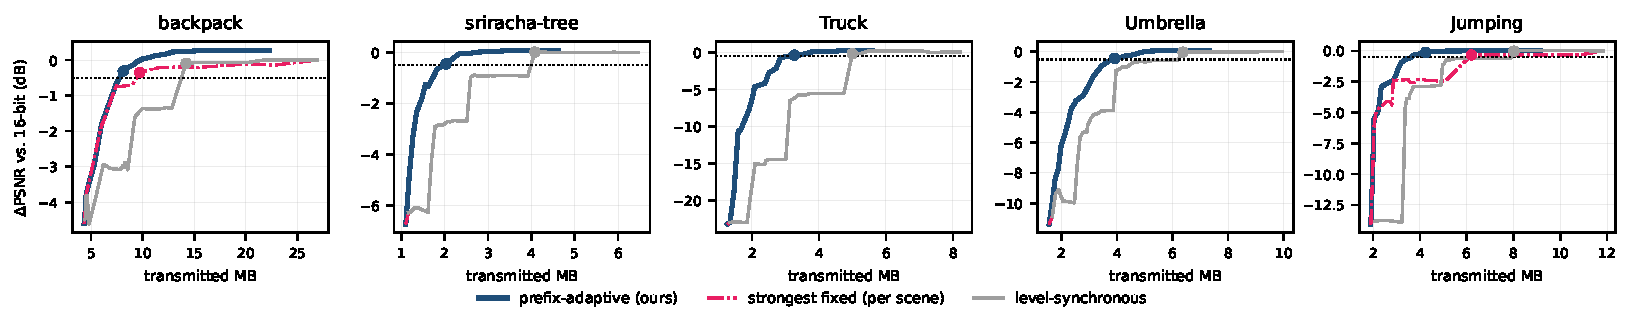
\includegraphics[width=\textwidth]{fig_firstplayable.pdf}
\caption{Quality of the first held-out frames as a function of the transmitted
bytes, relative to the 16-bit model, for three representative schedules: our
stream, the strongest fixed schedule of that scene, and the level-synchronous
order. The dotted line is the $-0.5$~dB target; dots mark where a schedule meets
both regional targets.}
\label{fig:prefix}
\end{figure*}

\begin{figure*}[t]
\centering
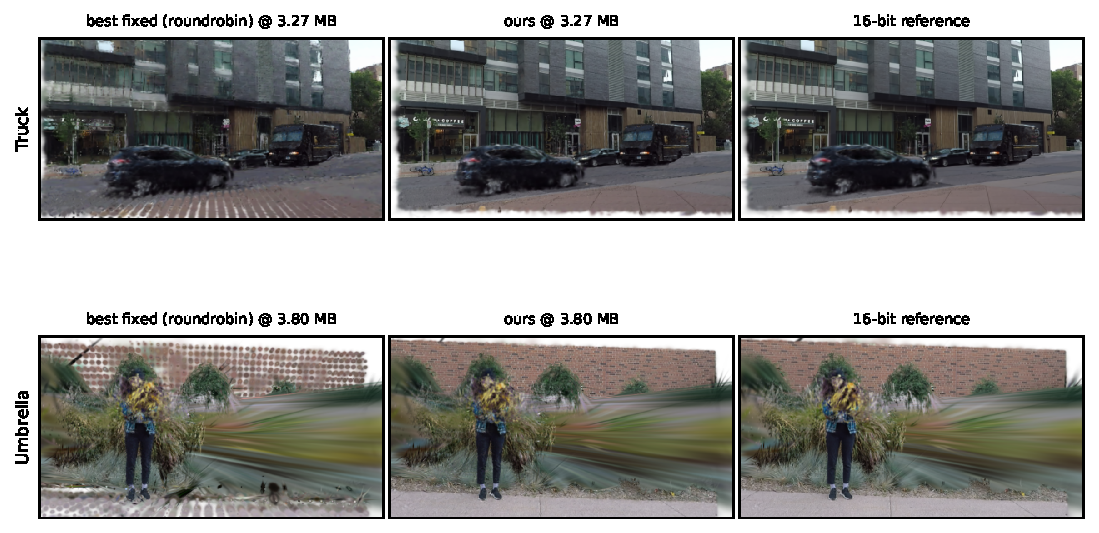
\includegraphics[width=\textwidth]{fig_samebudget_hero.pdf}
\caption{Visual quality under the same transmitted-byte budget. The strongest
fixed order and our stream are decoded at identical byte limits
($B_{\text{ours}}$ of the qualifying prefix); the 16-bit reconstruction is the
reference. All panels use the same held-out frame and camera and are shown
uncropped.}
\label{fig:hero}
\end{figure*}

\begin{figure*}[t]
\centering
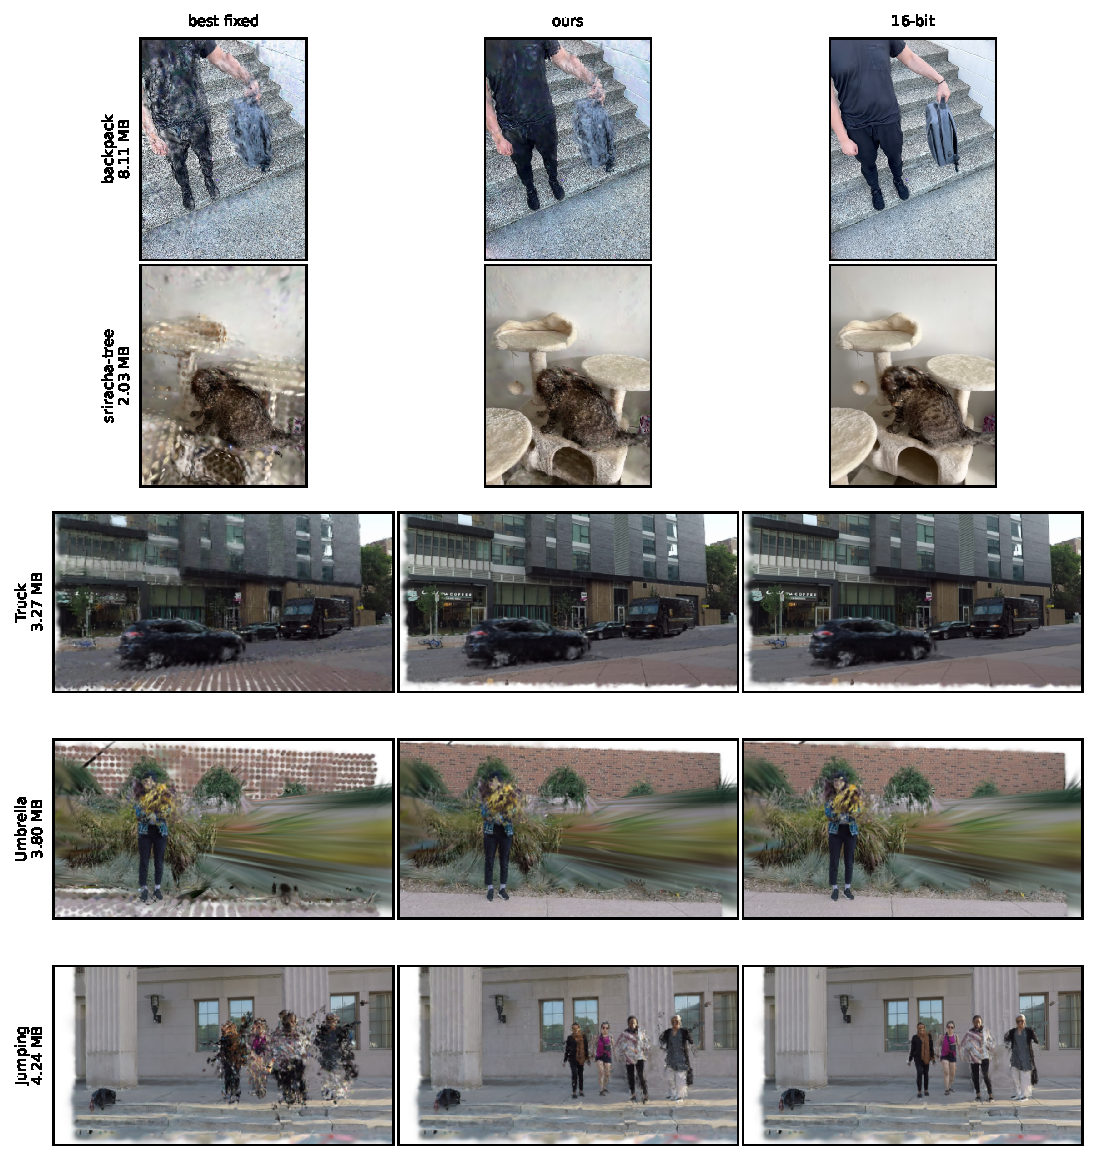
\includegraphics[width=\textwidth]{fig_samebudget_all.pdf}
\caption{Cross-scene comparison at matched transmitted bytes on the five
captures. Each row renders the same held-out frame with the strongest fixed
order, with our stream, and at 16-bit precision, at the budget where our stream
first satisfies both quality targets.}
\label{fig:allscenes}
\end{figure*}

\begin{figure*}[t]
\centering
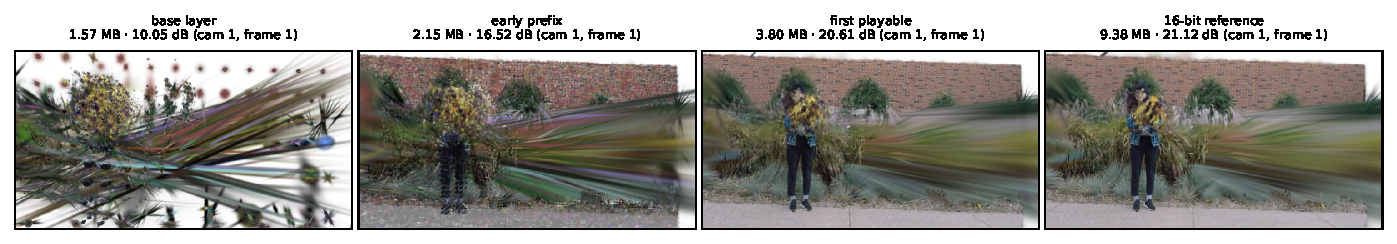
\includegraphics[width=\textwidth,height=0.235\textheight,keepaspectratio]{gallery_umbrella.pdf}\\[1pt]
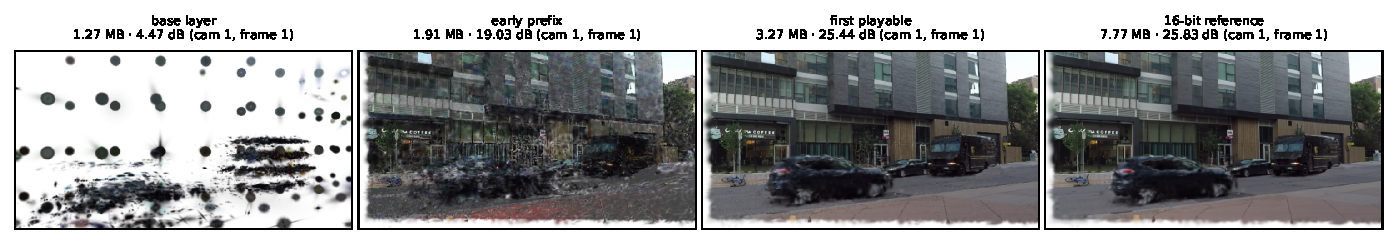
\includegraphics[width=\textwidth,height=0.235\textheight,keepaspectratio]{gallery_truck.pdf}\\[1pt]
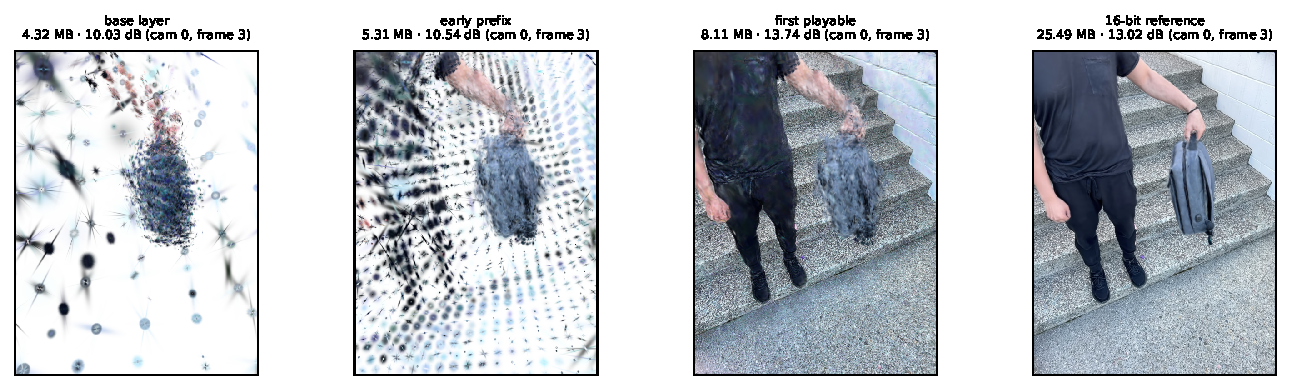
\includegraphics[width=\textwidth,height=0.235\textheight,keepaspectratio]{gallery_backpack.pdf}
\caption{Progressive delivery on three scenes, decoded from the actual packet
prefixes of the proposed order: base layer, an early prefix, the first-playable
prefix and the 16-bit reference. Each panel is a real decode of the same held-out
frame and is labelled with the masked PSNR \emph{of that frame} and its size: the
first three panels report the cumulative transmitted bytes of that prefix, while
the reference panel reports the $16$-bit payload size, which excludes packet
headers, the scale table and the camera blob. The tables report means over the
evaluation set.}
\label{fig:gallery}
\end{figure*}

\begin{table}[t]
\centering
\caption{Bytes to reach the dual-region first-playable threshold (MB of
transmitted data). The strongest fixed schedule is chosen per scene from the
six distinct schedules of \Cref{sec:baselines}; savings are computed from
unrounded byte counts. The level-synchronous column is the schedule that
\Cref{sec:baselines} also calls round-robin: once every schedule is expanded to
single packets the two produce the same sequence, so it is counted once.}
\label{tab:firstplayable}
\footnotesize
\setlength{\tabcolsep}{3.2pt}
\begin{tabular}{@{}lccccc@{}}
\toprule
Scene & base & \begin{tabular}[c]{@{}c@{}}level-\\sync\end{tabular} & best fixed & \textbf{ours} & \begin{tabular}[c]{@{}c@{}}save vs.\\best fixed\end{tabular}\\
\midrule
% generated by scripts/make_tex_tables.py
\emph{backpack} & 4.32 & 14.21 & 9.72 (m.p.) & \textbf{8.11} & 16.6\%\\
\emph{sriracha} & 1.10 & 4.08 & 4.08 (r.r.) & \textbf{2.03} & 50.3\%\\
\emph{Truck} & 1.27 & 5.00 & 5.00 (r.r.) & \textbf{3.27} & 34.6\%\\
\emph{Umbrella} & 1.57 & 6.38 & 6.38 (r.r.) & \textbf{3.80} & 40.4\%\\
\emph{Jumping} & 1.90 & 8.02 & 8.02 (r.r.) & \textbf{4.24} & 47.1\%\\
\bottomrule

\end{tabular}
\end{table}

\subsection{Where the ordering pays}
The gain tracks how far a scene's rate--distortion curve sits from saturation.
\emph{backpack} holds $87.1\%$ of its bytes in the background and its base
layer carries $53\%$ of the qualifying prefix, the setting in which an ordering
has the least room: it saves $16.6\%$. The other four scenes
concentrate quality in fewer groups, the qualifying prefix is a small multiple of
the base layer, and re-ordering pays $34.6$--$50.3\%$. The ranking of the fixed
schedules flips across scenes: the level-synchronous order is strongest in
every scene except \emph{backpack}, where multi-probe wins, and the frozen
single-score order is never the best, which is why the comparison
is made against the best fixed schedule rather than against a preferred one.

\subsection{Single stream across budgets}
One encoded stream has to serve clients whose budgets differ. We compare the
stream with an allocation optimised for each budget independently: a hill climb
on calibration frames over all groups and depths, started from the stream state
at that budget and from the base layer, priced by \eqref{eq:bytes} and scored on
the same calibration frames, with starts at the base layer and at the stream
state. \Cref{tab:scalable} reports fifteen matched budgets, three per scene;
across them the stream stays within $0.05$~dB of the locally optimised
per-budget allocation (mean
$-0.01$~dB on the full mask, $-0.00$~dB on the dynamic region). The allocation is a local optimum of a single-step hill
climb rather than a global one, and the stream matches it without being
re-optimised per budget. The same stream is monotone in received bytes; a ladder
of separately optimised models is not.

\begin{table}[t]
\centering
\caption{Single stream against a locally optimised allocation for the same
budget (masked PSNR in dB on evaluation frames; $\Delta$ is stream minus
allocation).}
\label{tab:scalable}
\scriptsize
\setlength{\tabcolsep}{3.0pt}
\begin{tabular}{@{}lccccccc@{}}
\toprule
Scene & MB & \begin{tabular}[c]{@{}c@{}}alloc.\\full\end{tabular} & \begin{tabular}[c]{@{}c@{}}stream\\full\end{tabular} & $\Delta_{\text{full}}$ & \begin{tabular}[c]{@{}c@{}}alloc.\\fg\end{tabular} & \begin{tabular}[c]{@{}c@{}}stream\\fg\end{tabular} & $\Delta_{\text{fg}}$\\
\midrule
% generated by scripts/make_tex_tables.py
\emph{backpack} & 9.78 & 13.90 & 13.91 & $+0.01$ & 12.95 & 12.94 & $-0.01$\\
 & 11.78 & 14.12 & 14.08 & $-0.04$ & 12.97 & 12.98 & $+0.01$\\
 & 14.59 & 14.21 & 14.21 & $+0.00$ & 12.98 & 12.98 & $-0.00$\\
\midrule
\emph{sriracha} & 2.53 & 16.78 & 16.77 & $-0.02$ & 13.83 & 13.79 & $-0.04$\\
 & 3.39 & 16.87 & 16.87 & $-0.00$ & 13.62 & 13.62 & $-0.00$\\
 & 4.33 & 16.89 & 16.89 & $+0.01$ & 13.61 & 13.62 & $+0.01$\\
\midrule
\emph{Truck} & 3.90 & 26.72 & 26.70 & $-0.02$ & 22.06 & 22.02 & $-0.04$\\
 & 4.93 & 26.81 & 26.81 & $-0.00$ & 22.26 & 22.23 & $-0.03$\\
 & 6.32 & 26.91 & 26.86 & $-0.04$ & 22.27 & 22.23 & $-0.05$\\
\midrule
\emph{Umbrella} & 4.58 & 21.29 & 21.29 & $-0.00$ & 19.92 & 19.92 & $-0.00$\\
 & 5.85 & 21.45 & 21.45 & $-0.00$ & 20.04 & 20.04 & $-0.00$\\
 & 7.34 & 21.46 & 21.46 & $-0.00$ & 20.06 & 20.06 & $+0.00$\\
\midrule
\emph{Jumping} & 5.06 & 24.19 & 24.19 & $+0.00$ & 19.68 & 19.68 & $+0.00$\\
 & 6.55 & 24.23 & 24.23 & $+0.00$ & 19.81 & 19.81 & $-0.00$\\
 & 8.49 & 24.24 & 24.24 & $+0.00$ & 19.81 & 19.81 & $+0.00$\\
\bottomrule

\end{tabular}
\end{table}


\subsection{Time-block split}
\label{sec:block}
Parity splitting leaves neighbouring frames on both sides of the split, so we
also calibrate on the first third of each sequence and evaluate on the last
third, with no frame from the middle and with the split taken on timestamps so
that each camera keeps its own frames. The packet sequence adapts to the
split---the first divergence comes between packet $2$ and packet $10$---and the
qualifying prefix moves by at most $1.34$~MB: the stream needs $8.13$, $1.69$,
$3.27$, $3.80$ and $2.90$~MB against $9.74$, $4.08$, $5.00$, $6.38$ and $4.97$~MB
for the strongest fixed schedule, that is $16.5\%$, $58.6\%$, $34.6\%$, $40.4\%$
and $41.6\%$ fewer bytes on the five scenes. The advantage therefore rides on the
calibrated objective, which re-estimates at every packet, rather than on a script
tied to one frame split.

\subsection{What the threshold means per frame}
\label{sec:frames}
The first-playable prefix is defined on the mean PSNR over the evaluated frames,
and a mean hides spread. At the qualifying prefix the per-frame full-mask PSNR
has a standard deviation of $0.26$--$3.31$~dB, and between $11\%$ and $53\%$ of
the individual frames sit below the mean threshold: the criterion is the mean over
the evaluated frames. Applying the threshold
to every frame instead, each against its own 16-bit value, needs $10.12$,
$2.71$, $3.68$, $4.32$ and $4.46$~MB, which is $24.9\%$, $33.7\%$, $12.8\%$,
$13.7\%$ and $5.3\%$ more than the mean criterion.
Measured against the captured video rather than against the checkpoint, our
qualifying prefix reaches PSNR $13.7$--$26.3$~dB, SSIM $0.34$--$0.78$ and LPIPS
$0.14$--$0.51$ over the five captures; on the two handheld captures the $16$-bit
model itself sits at
$14.0$ and $16.8$~dB, so the $-0.5$~dB criterion is a statement about the frozen
reconstruction's own fidelity, and the absolute numbers are what a deployment
inherits from that reconstruction. Both numbers are reported because a deployment chooses between them. Which
criterion the ranking serves matters here: a variant whose score is the $90\%$ empirical CVaR of the per-frame shortfall over
the twelve calibration frames (the weighted mean of the worst $1.2$ frames, against
each frame's own $16$-bit reference minus the tolerance), leaving the mean
criterion unchanged at the qualifying prefix, reaches the $90\%$-of-frames threshold on \emph{Jumping} at $4.80$~MB
instead of $11.38$~MB, while on the other four captures it moves that threshold by
$-0.19$ to $+0.71$~MB. The advantage is tied to this objective and this capture:
under the timestamp split all three orders qualify at the same bytes, so this is
a target to select for tail-sensitive delivery rather than a default. The five-scene table is in the
supplementary material.

\subsection{Cross-view consistency}
\label{sec:crossview}
Calibration uses twelve held-out frames of a single view: camera~1 on the three
multi-camera captures and the only view on the two monocular ones. On the
multi-camera captures the evaluation set then mixes cameras 1--3 in equal parts,
so \emph{Truck}, \emph{Umbrella} and \emph{Jumping} each judge $20$ of their $30$
frames on cameras 2 and 3, which never enter calibration.
\Cref{fig:crossview} renders one timestamp from cameras 1, 2 and 3 at the
first-playable prefix and at 16-bit precision: the moving subjects and the scene
geometry stay consistent across views at the delivered prefix, and the remaining
difference to the reference is in texture rather than in layout.

\subsection{Motion is preserved, not just the still frame}
\label{sec:motion}
Static PSNR says little about whether the dynamic content still moves as
captured. As a downstream proxy we render consecutive frames at the same camera
at the qualifying prefix, take the frame-difference magnitude over the dynamic
region, and correlate it with the ground-truth frame differences. The Pearson
correlation at the qualifying prefix is $0.53$, $0.87$, $0.63$, $0.15$ and
$0.41$ on \emph{backpack}, \emph{sriracha}, \emph{Truck}, \emph{Umbrella} and
\emph{Jumping}, against $0.71$, $0.94$, $0.67$, $0.16$ and $0.38$ for the
16-bit reconstruction: where the motion happens is largely recovered at the first playable prefix on
four of the five captures, with the gap visible mainly on \emph{backpack}. The
correlation reports how much of the motion survives at the delivered prefix.

\begin{figure*}[t]
\centering
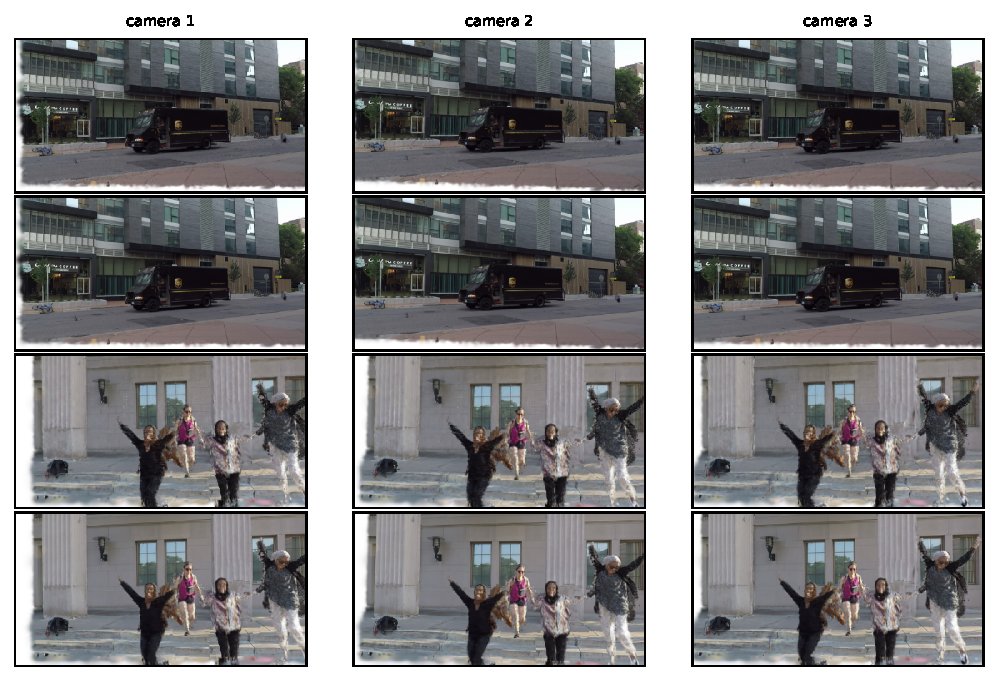
\includegraphics[width=\textwidth]{fig_crossview.pdf}
\caption{Same timestamp, three synchronised cameras, decoded from the first-playable
prefix (top of each pair) and from the 16-bit reconstruction (bottom). The scene
geometry and the moving subjects stay consistent across views, so the delivered
prefix holds on cameras whose frames never entered the calibration set.}
\label{fig:crossview}
\end{figure*}

\subsection{Runtime and overhead}
\label{sec:runtime}
Ordering is a producer-side cost paid once per scene: the calibration sweep
renders $5064$--$5328$ candidate prefixes, which takes about $100$--$170$~s on one
NVIDIA L40 for the five scenes, against a one-off encode of the base layer and
its packets. The client pays only entropy decoding of the packets it receives, and each
packet is individually framed; successive refinements of a group form a chain, so
a lost packet delays the remaining refinements of that group rather than the
other groups. Transmission dominates startup: the base layer
of \emph{backpack} is $4.32$~MB, which is $17.3$~s at $2$~Mb/s.

\subsection{Ablations}
\label{sec:ablation}
\label{sec:lambda}

\emph{Weight of the dynamic region.} \Cref{sec:utility} uses $\lambda=1$. Varying
$\lambda\in\{0,0.5,2\}$ moves the qualifying prefix by at most $0.21$~MB on any
scene ($8.11$ for all four weights on \emph{backpack}, $4.24$ on \emph{Jumping},
$2.03/1.84/1.82/2.13$ on \emph{sriracha}, $3.27/3.47/3.27/3.27$ on
\emph{Truck}, $3.80/3.80/3.87/3.80$ on \emph{Umbrella}). The qualifying byte
count is therefore insensitive to how the two regions are weighted, which is what
the dual-region acceptance test is for: it decides playability on its own terms,
while $\lambda$ only reweights the ranking that leads there.

\emph{What the score contributes.} The comparison above changes only the order.
Two further schedules re-estimate at every packet on the same candidates, ledger
and acceptance test, differing only in what they rank: the full-mask gain per byte, or the sum of the two regional gains.
\Cref{tab:adaptive} reports them. Three of the five scenes qualify at identical
bytes; \emph{Truck} favours the proposed score by $0.17$~MB and \emph{sriracha}
the full-mask gain by $0.19$~MB. The ordering holds across tolerances: moving the target over
$0.25$--$1.0$~dB shifts the qualifying prefix by at most $0.90$~MB. Which
schedule is shortest is itself tolerance-dependent, by $0.03$--$0.04$~MB: the
full-mask gain takes the lead on \emph{Truck} at $1.0$~dB, and the tail-aware
variant takes it on \emph{Umbrella} at the same tolerance. The choice of score therefore moves the qualifying
prefix by at most $0.19$~MB, while all three stay $16.6$--$55.0\%$ below the
strongest fixed schedule: the saving is associated with re-estimating at every
packet under the same transmitted-byte ledger. The ranking objective determines
the refinement order, while the dual-region acceptance criterion determines when
a prefix qualifies.


\begin{table}[t]
\centering
\caption{Bytes to reach the dual-region first-playable threshold (MB) for three
schedules that re-estimate at every packet and differ only in the ranking
objective, next to the strongest fixed schedule of each scene. All three share
the candidate packets, the byte ledger, the calibration and evaluation frames,
and the dual-region acceptance test. Bold marks the lowest byte count in each row,
ties included.}
\label{tab:adaptive}
\footnotesize
\setlength{\tabcolsep}{3.2pt}
\begin{tabular}{@{}lcccc@{}}
\toprule
Scene & \begin{tabular}[c]{@{}c@{}}best\\fixed\end{tabular} & \begin{tabular}[c]{@{}c@{}}full-mask\\gain\end{tabular} & \begin{tabular}[c]{@{}c@{}}joint\\gain\end{tabular} & \textbf{ours}\\
\midrule
% generated by scripts/make_tex_tables.py
\emph{backpack} & 9.72 & \textbf{8.11} & \textbf{8.11} & \textbf{8.11}\\
\emph{sriracha} & 4.08 & \textbf{1.84} & 2.03 & 2.03\\
\emph{Truck} & 5.00 & 3.44 & \textbf{3.27} & \textbf{3.27}\\
\emph{Umbrella} & 6.38 & \textbf{3.80} & \textbf{3.80} & \textbf{3.80}\\
\emph{Jumping} & 8.02 & \textbf{4.24} & \textbf{4.24} & \textbf{4.24}\\
\bottomrule

\end{tabular}
\end{table}
\emph{Second training seed.} Retraining every capture with a different seed
reproduces the comparison on all five: the direct order needs $8.32$, $2.02$,
$3.44$, $3.79$ and $4.22$~MB against $9.53$, $4.08$, $5.01$, $4.97$ and
$7.98$~MB for the strongest fixed schedule, that is $12.7$--$50.3\%$ fewer
bytes. The per-scene table is in the supplementary material.

\emph{Cross-camera calibration.} Calibrating on camera~2 and evaluating on
camera~1 leaves the qualifying prefix unchanged on \emph{Truck} ($3.27$~MB) and
\emph{Umbrella} ($3.80$~MB), and saves $0.07$~MB on \emph{Jumping} ($4.17$): the
ranking transfers between synchronised views of the same capture, moving the
prefix by at most $0.07$~MB on the three captures we tested.

\section{Discussion}
\label{sec:discussion}
The measurements predict where an ordering pays. When a scene's bytes sit in
groups that lose little at 4 bits, the base layer already carries much of the
qualifying prefix and there is little left for an order to win: \emph{backpack}
holds $87.1\%$ of its bytes in the background and saves $16.6\%$. When quality is
concentrated in a few groups, the qualifying prefix is a small multiple of the
base layer and re-ordering saves $34.6$--$50.3\%$. Both regimes are visible from a
single truncation sweep on the calibration frames, before any client is served.

The two kinds of policy differ in what they need. A linear sensitivity model
needs one sweep and no rendering of candidate prefixes, and it is the classic
choice; on our scenes it lands behind round-robin on three of five scenes,
because the marginal value of a group depends on how far the others already are.
The direct policy needs a few thousand calibration renders, once per scene, and
in exchange it re-reads the marginal value at every packet.

What this paper adds is measurement plus a delivery contract rather than new
machinery: byte share and sensitivity rank groups differently in a factorised 4D
model, the ranking flips with the scene, the transmitted-byte ledger is the real
serialized stream (every prefix size is the byte offset of that prefix, and the
decoder reproduces the 16-bit grid bit-exactly), and one stream stays within
$0.05$~dB of per-budget allocations at fifteen matched budgets while removing
$16.6$--$50.3\%$ of the startup bytes relative to the strongest fixed order.

For a streaming service the consequence is that the time-invariant part of a
reconstructed scene is worth sending once at high precision and caching on the
client, while the dynamic part is cheap to refresh: our measurements put the
dynamic share between $5.4\%$ and $33.4\%$ of the model. A client that caches the
background can start later sessions from the dynamic residual alone.

\section{Conclusion}
\label{sec:conclusion}
A frozen 4D Gaussian scene can be delivered progressively without retraining it:
encoded as a base layer plus bit-plane refinement packets, it becomes a single
truncatable stream whose completed prefixes decode and render as data arrives.
Ranking each packet by the shortfall it removes from the full-scene and
dynamic-region targets per transmitted byte turns the measurement of where the
bytes sit into a delivery order that reaches the first playable frames with
$16.6$--$50.3\%$ fewer bytes than the strongest of six distinct fixed schedules, while one
stream still serves a ladder of client budgets. The same one-off sweep that fixes the order
tells a producer, before any client is served, whether an adaptive order pays for
a given scene: a flat curve saturates early and needs no ordering, a steep one
hands the startup bytes to a per-packet schedule.

\section*{Use of Generative AI}
\label{sec:genai}
Generative AI tools were used to polish the language of this manuscript: they
suggested wording, grammar and readability improvements to text drafted by the
authors. The problem formulation, the protocol, the ordering rule, the
implementation, the experiments and every reported number are the authors' own
work; the authors verified all text and take full responsibility for the content
of this paper.

\appendices
\section{Reproduction}
\label{app:repro}
All numbers in this paper are produced by the scripts listed below from the
checkpoints used in our experiments, on a single NVIDIA L40. The companion
package supports a reader without those weights: every table, byte count and
statistic in this paper can be recomputed from the stored JSON in it.
Re-rendering the PSNR values or regenerating a checkpoint needs the original
captures and the model weights, which are not redistributed.
\textbf{(1) Structure:} \texttt{r4d\_rates.py} tabulates entropy-coded sizes per
attribute group and bit depth; \texttt{packets.py --selftest} verifies the
serializer and decoder bit-exactly; \texttt{sens\_grid.py} renders the
single-group truncation table on the calibration frames of the $16$-bit grid.
\textbf{(2) Orders:} \texttt{r4d\_prefix.py} builds every delivery order, writes
the real packet sequence, asserts that each recorded size equals the byte offset
of the prefix in that stream, and records the masked PSNR of the first held-out
frames with the cumulative size. \texttt{alloc\_search\_p0.py} optimises an
allocation for a fixed budget under the same byte ledger.
\textbf{(3) Verification:} \texttt{check\_numbers.py} re-derives every number
quoted in the text from the stored artefacts and \texttt{audit\_numbers.py}
re-derives the prefix sizes, the sensitivity matrix and the matched-budget
differences independently of the table generator.

\clearpage
\bibliographystyle{IEEEtran}
\bibliography{refs}

\end{document}
